\documentclass[12pt]{article}

\usepackage[skip=10pt plus1pt, indent=0pt]{parskip}
\usepackage{multicol}
\usepackage{listings}
\usepackage{amsmath}
\usepackage{verbatim}
\usepackage{subcaption}
\usepackage{bookmark}
\usepackage{graphicx}
\usepackage{hyperref}
\usepackage{xcolor}

\usepackage{color}
\definecolor{codegreen}{rgb}{0,0.6,0}
\definecolor{codegray}{rgb}{0.5,0.5,0.5}
\definecolor{codepurple}{rgb}{0.58,0,0.82}
\definecolor{backcolour}{rgb}{0.95,0.95,0.92}

\lstdefinestyle{mystyle}{
    backgroundcolor=\color{backcolour},
    commentstyle=\color{codegreen},
    keywordstyle=\color{magenta},
    numberstyle=\tiny\color{codegray},
    stringstyle=\color{codepurple},
    basicstyle=\ttfamily\footnotesize,
    breakatwhitespace=false,
    breaklines=true,
    captionpos=b,
    keepspaces=true,
    numbers=left,
    numbersep=5pt,
    showspaces=false,
    showstringspaces=false,
    showtabs=false,
    tabsize=2
}

\lstset{style=mystyle}


\title{\textbf{SENG 474: Data Mining \\Assignment 3} \\[2ex]
\large Clustering Experiments: 
\large \textit{Lloyd's Algorithm and Hierarchical Agglomerative Clustering}}
\author{Sean McAuliffe, V00913346 (A02)}
\date{March 23\textsuperscript{rd}, 2023 AD}
\graphicspath{{../figures/}}

\begin{document}

\maketitle

\pagebreak
\tableofcontents  
\pagebreak

\section{Introduction}

This report summarized the results obtained from applying two 
clustering algorithms, Lloyd's Algorithm and Agglomerative Clustering to two
provided datasets. The first dataset contains 3500 points in 2 dimensions, and
the second dataset contains 14801 points in 3 dimensions. The purpose of this
exercise is to gain familiarity with implementing clustering algorithms, and to
gain an understanding of the differences between approaches; in order to be
able to interpret their results, choose an appropriate number of clusters for
a given problem and apply appropriate solutions for different situations.

Clustering is an unsupervised learning technique with the goals of
categorizing data into groups based on their similarity. In this way, labels 
can be learned from the data itself; without the need for pre-labelled data.
Clustering is a useful technique in data mining which can be used to find 
patterns in datasets, perhaps as a pre-processing step for further supervised
learning methods. The notion of a cluster is not easy to formalise (one 
recognises a cluster when one sees it). Accordingly, many algorithms exist for
producing clusterings from data.

\section{Implementation}

The experiments conducted for this report were composed in an accompanying
Jupyter notebook running on a \emph{Python 3.10.6} Kernel. An implementation of
Lloyd's algorithm was written for this assignment, according to the description
provided in the lecture 23 slides. An implementation of agglomerative clustering
was imported from the \emph{sci-kit learn} library. The
\emph{sklearn.cluster AgglomerativeClustering} class was used, which provides
the necessary connectivity metrics for determining the distance between
clusters. 

All code for implementation of the algorithms, use of external libraries, data
loading, and graph generation is contained in the accompanying Jupyter notebook.

\subsection{Provided Datasets}

In order to build an intuition for the behaviour of the algorithms in later
experiments, the provided data were plotted in 2 and 3 dimensions respectively.
This is shown in Figure \ref{fig:provided_data}.

\begin{figure}[h]
    \centering
    \begin{subfigure}{0.3\textwidth}
      \centering
      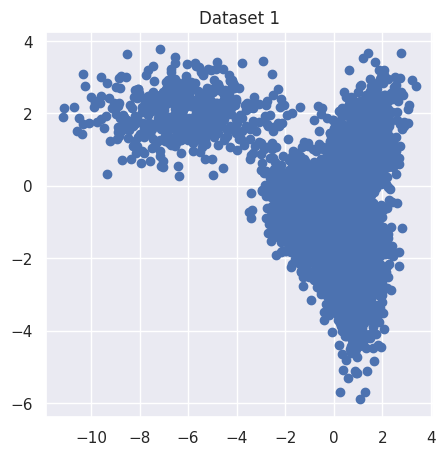
\includegraphics[width=\linewidth]{0.png}
      \caption{Dataset 1, 2D}
      \label{fig:provided_data_1}
    \end{subfigure}%
    \hfill
    \begin{subfigure}{0.3\textwidth}
      \centering
      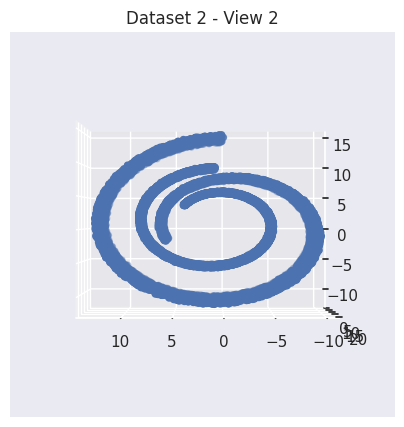
\includegraphics[width=\linewidth]{00.png}
      \caption{Dataset 2, 3D}
      \label{fig:provided_data_2}
    \end{subfigure}%
    \hfill
    \begin{subfigure}{0.3\textwidth}
      \centering
      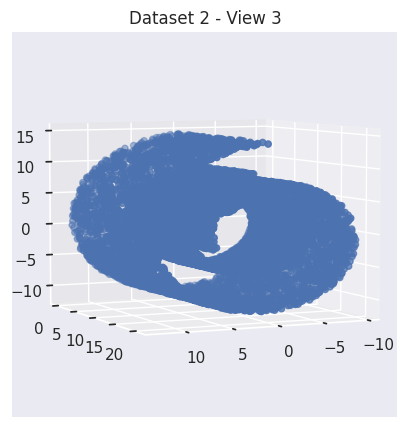
\includegraphics[width=\linewidth]{000.png}
      \caption{Dataset 2, 3D}
      \label{fig:provided_data_3}
    \end{subfigure}
    \caption{The shape of the provided datasets in 2 and 3 dimension}
    \label{fig:provided_data}
\end{figure}

The first dataset seems like it ought to be seperable into roughly 2 clusters.
The clusters seem to be globular, but clearly oblong. The second dataset
seems to also be seperable into 2 clusters, however it is highly non-globular.
Rather, it is composed of two intertwined spirals having the appearance of a
dessert.

\section{Lloyd's Algorithm}

\textbf{Lloyd's algorithm} is a k-means clustering algorithm in which 
clusters are defined by the mean of the points in the cluster. Lloyd's algorithm 
is an iterative algorithm which converges on a clustering of minimum cost by 
repeatedly assigning points to their nearest clusters, and then recomputing the
cluster means, until the assignments of points to clusters no longer changes.
Through this process, the means which describe a clustering are learned. 

The algorithm is as follows:

\begin{enumerate}
    \item Initialise the means of the clusters (using one of the below methods)
    \item Assign each point to the cluster with the nearest mean.
    \item Recompute the means of the clusters.
    \item Repeat steps 2 and 3 until the assignments of points to clusters no
    longer changes.
\end{enumerate}

The goal is to learn a minimum-cost clustering of the dataset into \textit{k}
clusters. The cost of a k-clustering, \textit{C} is defined as:

\begin{equation}
    W(C) = \sum_{j=1}^{k} \sum_{x \in C_j} \lVert x - \mu_j \rVert^2
\end{equation}

This assignment required Lloyd's algorithm to be implemented, the implementation
is shown in the code snippet below.

\begin{lstlisting}[language=Python]
def lloyd(X, k, init):
    # Initialize the clusters
    C = init(X, k)
    # Repeat until the centres do not change
    previous_centres = get_centres(C)
    i = 0
    while True:
        i += 1
        # Assign each data point to the cluster with the closest centre
        for cluster in C:
            cluster.clear_data()
        assign_to_closest(X, C)
        # Update the cluster centres
        for cluster in C:
            ideal_centre = np.mean(cluster.data, axis=0)
            # Find the point in the data closest to the idealized centre
            min_dist = np.inf
            min_point = None
            for point in cluster.data:
              dist = euclidean_distance(point, ideal_centre)
                if dist < min_dist:
                    min_dist = dist
                    min_point = point
            cluster.centre = deepcopy(min_point)
        # Check if the centres have changed
        new_centres = get_centres(C)
        if all_centres_equal(previous_centres, new_centres):
            break
        previous_centres = new_centres
    return i, C
\end{lstlisting}

\subsection{Initialisation}

The algorithm is probabilistic in that the initialisation of the means is
probabilistic, and so the algorithm may converge to a different clustering each
time it is run, and each run may require a variable number of iterations to
converge. To find a low cost clustering it may be necessary to run the algorithm
multiple times, and to choose the clustering with the lowest cost. 

\textbf{Uniform random initialisation} is a method of initialising the means of the
clusters by randomly sampling, without replacement, points from the dataset with
equal probability. This method is simple to implement, however it can lead to
poor results and poor runtimes if the initial means are poorly chosen.

\textbf{K-Means++ Initialisation} proceeds from the notion that cluster centres
ought not to be near to each other, as such points are likely to be assigned to
the same cluster. K-Means++ initialisation can reduce runtime by preferring to
sample points which are far from the current cluster centres. The first cluster
centre is chosen uniformly at random from the dataset, subsequent centres are
chosen with probability proportional to the squared distance from the nearest
cluster centre. This method is more likely to produce good results than uniform
random initialisation, resulting in lower expected runtimes.

This assignment involved implementing k-means++ initialisation, a snippet
showing part of the implementation is below.

\begin{lstlisting}[language=Python]
for x in X:
  min_dist = np.inf
  for cluster in clusters:
    dist = cluster.distance(x)
    if dist < min_dist:
      min_dist = dist
      dists.append(min_dist)
  probability_vector = dists/np.sum(dists)
  centre = X[np.random.choice(len(X), p=probability_vector)]
\end{lstlisting}

\subsection{The Elbow Method}

Determining how many clusters are present in a dataset is a difficult problem
to formalise. Instead, for this assignment the elbow method was used to determine
the proper number of clusters to use. The elbow method is a heuristic method
in which the number of clusters, \emph{k} is incremented, and a clustering algorithm is
run to produce a clustering for each \emph{k}. The cost of each k-clustering
is measured (for each \emph{k} the algorithm is run multiple times and the lowest
cost clustering is chosen as the result). The cost of each k-clustering is
plotted as a function of k. The resulting plot should contain a steadily decreasing
curve, ideally with a sharp bend at the point of diminishing returns. The point
at which the curve bends is the optimal number of clusters to use.

\subsection{Experimental Results}

\subsubsection{Lloyd's Algorithm on Dataset 1}

The number of clusters was varied from [2, 10] and for each value of \emph{k} the
algorithm was run 10 times, and the lowest cost clustering was chosen as the
result. For each of the chosen clusterings, its cost and the number of iterations
required to converge were recorded. The results are shown in \ref{fig:elbow_1}

\begin{figure}[h]
    \centering
    \begin{subfigure}{0.5\textwidth}
      \centering
      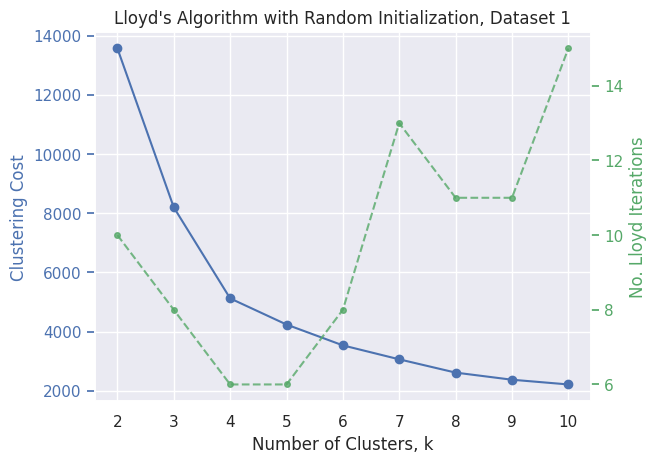
\includegraphics[width=\linewidth]{4.png}
      \caption{Random Initialisation}
      \label{fig:4}
    \end{subfigure}%
    \hfill
    \begin{subfigure}{0.5\textwidth}
      \centering
      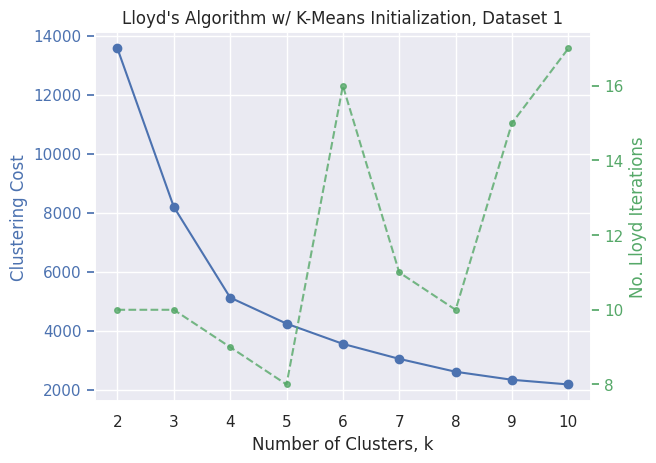
\includegraphics[width=\linewidth]{6.png}
      \caption{K-Means++ Initialisation}
      \label{fig:6}
    \end{subfigure}%
    \caption{The elbow method graph for dataset 1}
    \label{fig:elbow_1}
\end{figure}

One thing to notice is that the results are very similar. Indeed, the cost of the
clusterings chosen for each value of k are almost identical. In both plots, there
appears to be an elbow that appears sharpest at k = 4. This choice is somewhat
arbitrary, and sensitive to such things as the presented scale of the axes.

Another thing to notice is that the number of iterations required to converge increases
sharply after the elbow-point. And, that k-means++ initialisation did not appear to
significantly reduce the number of iterations required to converge. This is likely
due to the small size of the dataset, with so few points and clusters, the initialisation
is very sensitive to the choice of initial means.

\begin{figure}[h]
    \centering
    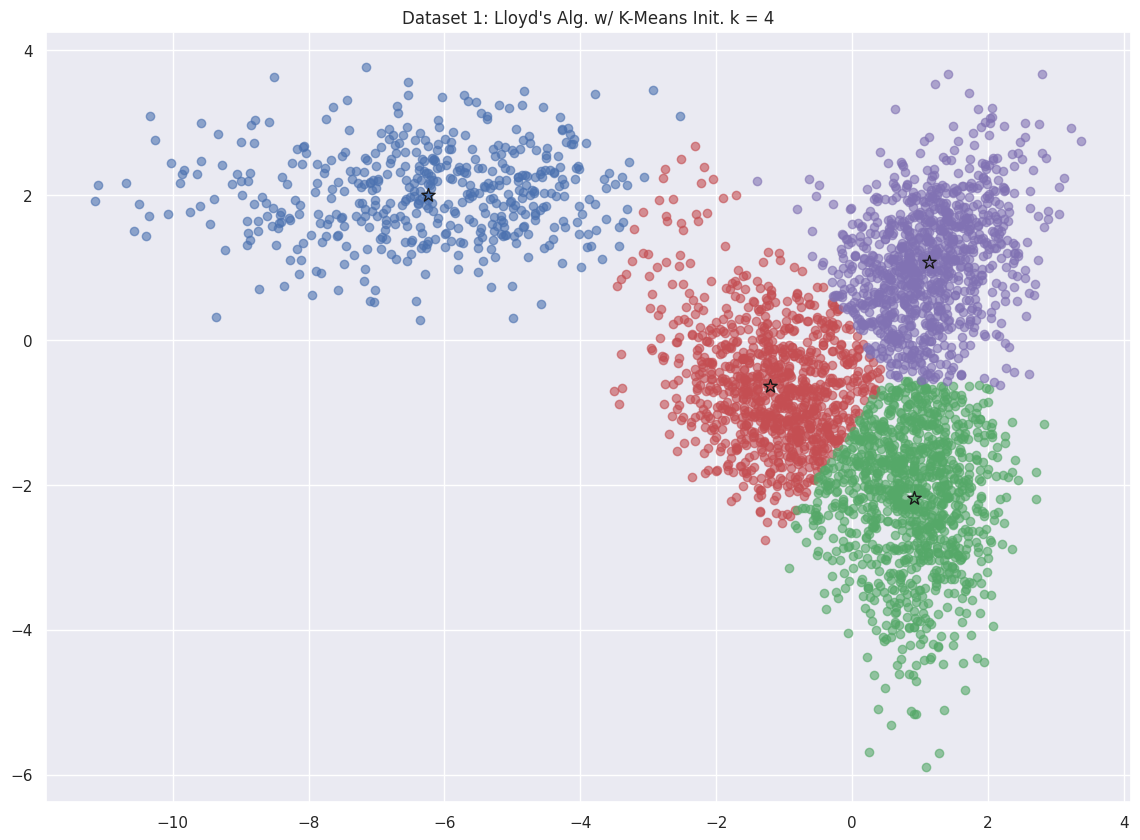
\includegraphics[width=\linewidth]{7.png}
    \caption{Clustering produced by Lloyd's Algorithm w/ k = 4}
    \label{fig:dist_1}
\end{figure}

\section{Hierachical Agglomerative Clustering}

\textbf{Hierarchical agglomerative clustering} is a connectivity-based
algorithm in which clusters are defined by their member points (depending on the
coonectivity, or linkage, metric used). The algorithm begins by assigning each
point to its own cluster. Then, at each iteration, the two clusters with the
smallest distance between them are merged together. This process is repeated 
until the desired number of clusters is reached.

\end{document}